\subsubsection{Materials}
\begin{itemize}
    \item Hot plate, digital thermocouple.
    \item Magnetic stirrer.
    \item Cotton wool, aluminium foil.
    \item Plastic cup.
\end{itemize}
\subsubsection{Method} \label{sec:Heating-method}
Five comparative experiments were designed to investigate heat flux under various conditions, considering of the following aspects:
\begin{enumerate}
    \item Experiment 1:  Compare the temperature range within the reactor under mixing condition and non-mixing condition, both without insulation. 
    \item Experiment 2: Compare the temperature range within the reactor with insulation and without insulation, both under mixing condition. 
    \item Experiment 3: Compare cotton and aluminium foil to decide which should be used for insulation in the final prototype. 
    \item Experiment 4: Compare the temperature range within the reactor with 1cm thick cotton insulation and 2 cm thick cotton insulation.
    \item Compare the addition of an Aluminum lid versus no lid on top of the vessel.
\end{enumerate}

\paragraph{General procedures:}
\begin{enumerate}
    \item Set the hot plate to \SI{35}{\celsius}.
    \item Fill up the vessel with \SI{300}{\milli\litre} of water.
    \item Take radial measurements at 0 cm, 1.5 cm and 3 cm from the center of the vessel with a vertical distance of 7.5 cm.
    \item Take vertical measurements at 1.5 cm, 4.5 cm and 7.5 cm from bottom of the vessel.
\end{enumerate}

The apparatus was set up according to Figure \ref{fig:Heating-setup}

\begin{figure}[h]
    \centering
    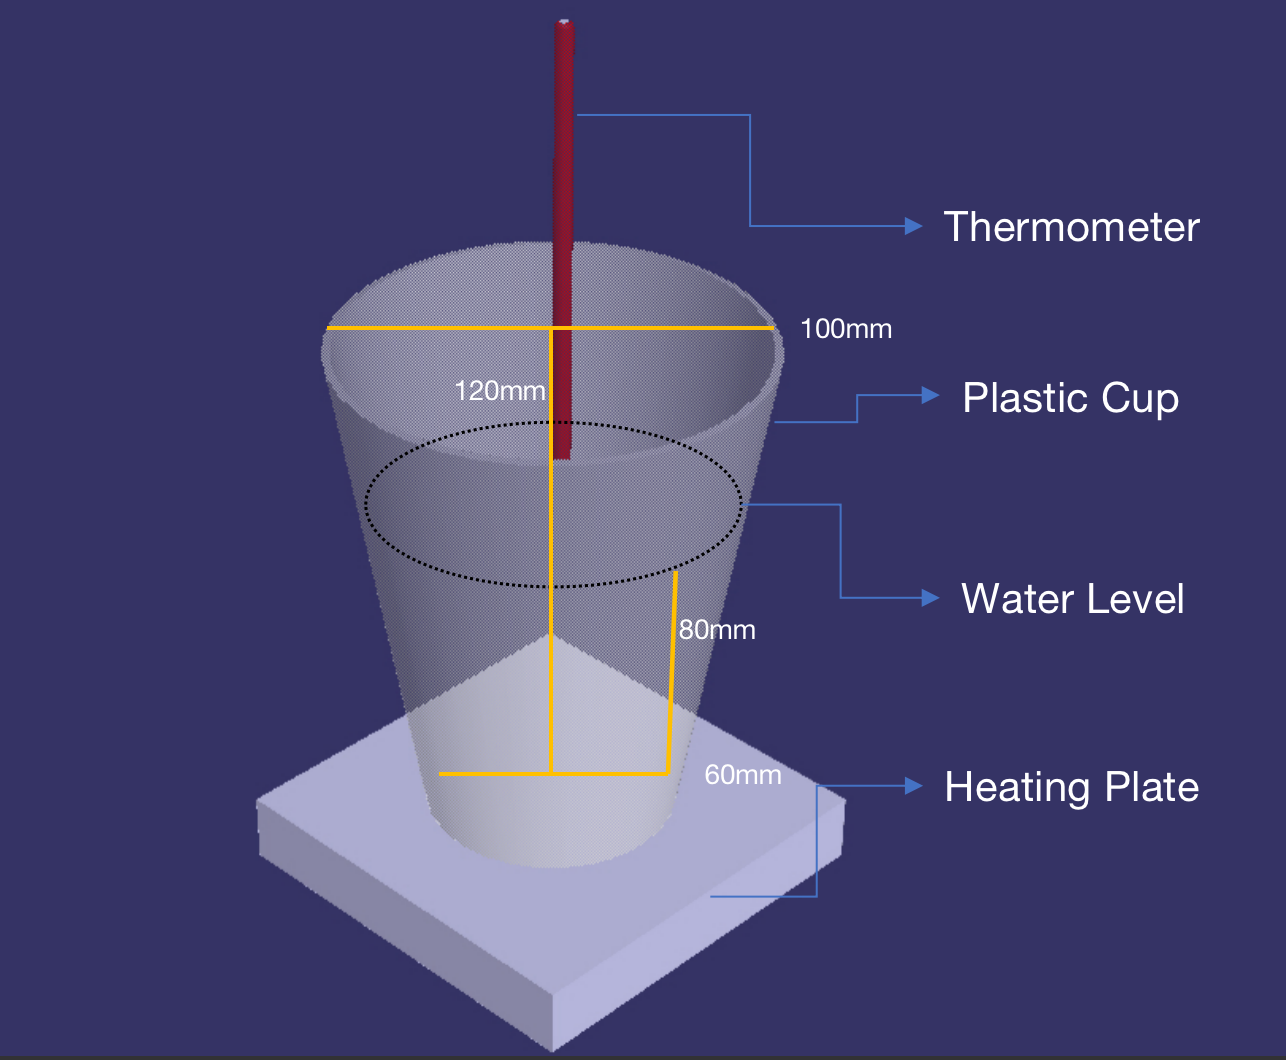
\includegraphics[width=0.40\textwidth]{Heating-cup.png}
    \caption{Apparatus setup}
    \label{fig:Heating-setup}
\end{figure}